%%%%%%%%%%%%%%%%%%%%%%%%%%%%%%%%%%%%%%%%%%%%%%%%
%
%	NOTATIONS
%
%%%%%%%%%%%%%%%%%%%%%%%%%%%%%%%%%%%%%%%%%%%%%%%%



% Commandes g�n�rales
%===============================


%Lettres grecques oubliees
\newcommand{\Mu}{M} %mu majuscule

%Mise en forme
\newcommand{\gras}[1]	{\textbf{#1}}
\newcommand{\bouton}[1]	{\fbox{\footnotesize{\textsc{#1}}}}
\newcommand{\toutpetit}[1]	{{\tiny{1}}}
\newcommand{\PETIT}[1]		{{\scriptsize{#1}}}
\newcommand{\Petit}[1]		{\footnotesize{#1}}
\newcommand{\petit}[1]		{{\small{#1}}}
\newcommand{\normal}[1]		{{\normalsize{#1}}}
\newcommand{\grand}[1]		{{\large{#1}}}
\newcommand{\Grand}[1]		{{\Large{#1}}}
\newcommand{\GRAND}[1]		{{\LARGE{#1}}}
\newcommand{\enorme}[1]		{{\huge{#1}}}
\newcommand{\Enorme}[1]		{{\Huge{#1}}}

\newcommand{\oeuvre}		{\oe uvre}
\newcommand{\oeuvres}		{\oe uvres}

\newcommand{\fig}[1]		{(fig.\ref{#1})}

\newcommand{\miniCentre}[2][\linewidth]	{\begin{minipage}{#1}\begin{center}#2\end{center}\end{minipage}}


%NOTATIONS PAR THEME
%%%%%%%%%%%%%%%%%%%%%%%%


%%%%%%%%%%%%%%%%%%%%%%%%%%%
%
% Notations math�matiques
%
%%%%%%%%%%%%%%%%%%%%%%%%%%%%%%%

\newcommand{\ssi}{si et seulement si }
\newcommand{\indiceGauche}[2]	{\ensuremath{	{\vphantom{#2}}_{#1}{#2} 	}}
\newcommand{\exposantGauche}[2]	{\ensuremath{	{\vphantom{#2}}^{#1}{#2} 	}}
\newcommand{\transposee}[1]	{\ensuremath{	\exposantGauche{\mathit t}{#1}	}}%{\vphantom{#1}}_{\mathit t}{#1}	}}

% FONCTION
%%%%%%%%%%%%%%%%%%%%
\newcommand{\fonction}[2]	{\ensuremath{	{#1}_{\left(#2\right)}		}}
\newcommand{\f}[2]		{	\fonction{#1}{#2}		}
\newcommand{\deriv}[3][]	{\ifthenelse{\equal{#1}{}}	{\ensuremath{	\frac{d{#2}}{d{#3}}}}	{\ensuremath{	\left[\frac{d{#2}}{d{#3}}\right]_{#1}}}}
\newcommand{\atan}[1][]		{\ifthenelse{\equal{#1}{}}	{\ensuremath{	\tan^{-1}	}}	{\ensuremath{	\tan^{-1}\left(#1\right)	}}}


% ENSEMBLES
%%%%%%%%%%%%%%%%%%%%%%%%%%%%%%
\newcommand{\R}		{\ensuremath{\mathbb{R}}	}
\newcommand{\couple}[2]{\ensuremath{\left(#1,#2\right)}}	%Couple (ex : (U,V) )
\newcommand{\triplet}[3]{\ensuremath{\left(#1,#2,#3\right)}}	%Triplet (ex : (U,V,W) )
\newcommand{\quadruplet}[4]{\ensuremath{\left(#1,#2,#3,#4\right)}}	%Triplet (ex : (U,V,W) )



% GEOMETRIE
%%%%%%%%%%%%%%%%%%%%%%%%%%
\newcommand{\segment}[1]	{\ensuremath{	\left[#1\right]		}}		%Fait un sement
\newcommand{\droite}[1]		{\ensuremath{	\left(#1\right)		}}
\newcommand{\arc}[1]		{\ensuremath{	\overset{\frown}{#1}	}}		%Arc
\renewcommand{\angle}[1]	{\ensuremath{	\left(\widehat{#1}\right)	}} %(Red�fini : la fonction angle correspondait au symbole angle)
%%%%%%%%%%%%%%%%%%%%%%%%%%%%%%%%%%%%%%%%%%
%	unit�s
%%%%%%%%%%%%%%%%%%%%%%%%%%%%%%%%%%%%%%%%%%


\newcommand{\unite}[1]	{{\,\PETIT{\ensuremath{	\color{black}\text{#1}	}}}}

%Longueurs
\newcommand{\mm} 	{\unite{mm}}
\newcommand{\cm} 	{\unite{cm}}
\newcommand{\m} 	{\unite{m}}
\newcommand{\dam} 	{\unite{dam}}
%\newcommand{\hm} 	{\unite{hm}}
\newcommand{\km} 	{\unite{km}}
\newcommand{\orto}{^{\circ}} %degre


%Forces
\newcommand{\N} 	{\unite{N}}
\newcommand{\daN} 	{\unite{daN}}
\newcommand{\Nm} 	{\unite{N\,m}}
\newcommand{\Pa} 	{\unite{Pa}}
\newcommand{\MPa} 	{\unite{MPa}}
\newcommand{\br} 	{\unite{bar}}


%Temps
\renewcommand{\sec} 	{\unite{s}}
\newcommand{\mn} 	{\unite{min}}
\newcommand{\h} 	{\unite{h}}

%Masse
\newcommand{\g} 	{\unite{g}}
\newcommand{\Kg} 	{\unite{Kg}}
%%%%%%%%%%%%%%%%%%%%%%%%%%%%%%%%%%%%%%%%%%%%
%
%	Notations Analyse fonctionnelle
%
%%%%%%%%%%%%%%%%%%%%%%%%%%%%%%%%%%%%%%%%%%%%


%Analyse fonctionnelle
\newcommand{\MO}	{mati�re d'\oe uvre}
\newcommand{\VA}	{valeur ajout�e}

%%%%%%%%%%%%%%%%%%%%%%%%%%%%%%%%%%%%%%%%%%%%
%
%	Notations asservissements
%
%%%%%%%%%%%%%%%%%%%%%%%%%%%%%%%%%%%%%%%%%%%%

%Automatique
\newcommand{\TOR}	{		tout-ou-rien	}
\renewcommand{\L}	{\ensuremath{	\mathscr{L}	}}	%Transform�e de Laplace (anciennement un L barr�)
%%%%%%%%%%%%%%%%%%%%%%%%%%%%%%%%%%%%%%%%%%%%
%
%	Notations vecteurs/torseurs
%
%%%%%%%%%%%%%%%%%%%%%%%%%%%%%%%%%%%%%%%%%%%%



%Commandes de base
%-----------------------------
\newcommand{\vecteur}[1]	{\ensuremath{	\protect\overrightarrow{#1}}}	%Fait un vecteur
\newcommand{\vecteurIndice}[2]	{\ifthenelse{\equal{#2}{\ }}{\vecteur{{#1}}\ }{\vecteur{{#1}_{#2}}}}	%Fait un vecteur avec un indice (x1, y1...), ou un vecteur simple si indice = espace
\newcommand{\vecteurChamp}[2]	{\fonction{\vecteur{#1}}{#2}}
\newcommand{\bipoint}[2]	{\ensuremath{	\vecteur{\segment{#1#2}}	}}	%bipoint
\newcommand{\vLie}[2]		{\ensuremath{	\couple{#1}{#2}	}}			%Vecteur lie
\newcommand{\vGlissant}[2]	{\ensuremath{	\couple{#1}{#2}	}}			%Vecteur glissant
\newcommand{\fN}[2][] {\ensuremath{	\protect\overrightarrow{N_{#1\rightarrow#2}}}}			%Vecteur lie
\newcommand{\fT}[2][]	{\ensuremath{	\protect\overrightarrow{T_{#1\rightarrow#2}}}}
\newcommand{\fpbis}	{\ensuremath{	\protect\overrightarrow{f_{p (S_1\rightarrow S_2)}}}}

%Espaces
%--------------------------------
\newcommand{\eAffine}[1][3]	{\ensuremath{	\mathscr{E}^{#1}	}}	%Espace affine
\newcommand{\eVectoriel}[1][3]	{\ensuremath{	E^{#1}			}}	%Espace vectoriel



%Repr�sentation des vecteurs
\newcommand{\vColonne}[2][]	{\ensuremath{	\left( \begin{array}{c} #2 \end{array} \right)_{#1}	}}	%Vecteur colonne (avec coordonn�es)


%Operateurs Vectoriel

\newcommand{\norme}[1]		{\ensuremath{	\left\Vert #1 \right\Vert	}}	%Norme
\newcommand{\abs}[1]		{\ensuremath{	\left\vert #1 \right\vert	}}	%Valeur absolue
\newcommand{\prodMixte}[3]	{\ensuremath{	\left(#1\wedge#2\right)\cdot#3	}}	%produit mixte
\newcommand{\doubleProdVect}[3]	{\ensuremath{	#1\wedge\left(#2\wedge#3\right)	}}	%produit vectoriel



%VECTEUR PRE-FAVRIQUES
%------------------------------


\newcommand{\vNul}		{\ensuremath{	\overrightarrow{0}	}}	%Symbole d'une base
\newcommand{\vPreFab}[2][]	{\ifthenelse{\equal{#1}{}}	{\vecteur{#2}}	{\vecteurChamp{#2}{#1}}	}	%Vecteur qui choisit tout seul si c'est un vecteur simple ou un champ (pr�sence d'un parametre ou non)


%Tout ce qui est vecteurs e_i
\newcommand{\ve}[1]{\vecteurIndice{e}{#1}}

\newcommand{\vex}{\ve{x}}	%e_x
\newcommand{\vey}{\ve{y}}	%e_y
\newcommand{\vez}{\ve{z}}	%e_z

%\newcommand{\e}{\ensuremath{\overrightarrow {e_2}}}
%\newcommand{\e}{\ensuremath{\overrightarrow {e_3}}}

\newcommand{\vx}[1]{\vecteurIndice{x}{#1}}	%x_i
\newcommand{\vy}[1]{\vecteurIndice{y}{#1}}	%y_i
\newcommand{\vz}[1]{\vecteurIndice{z}{#1}}	%z_i

%\newcommand{\vXzero}{\ensuremath{\vecteur{x_1}}}
%\newcommand{\vYun}{\ensuremath{\vecteur{y_1}}}
%\newcommand{\vZun}{\ensuremath{\vecteur{z_1}}}

%\newcommand{\vXun}{\ensuremath{\vecteur{x_1}}}
%\newcommand{\vYun}{\ensuremath{\vecteur{y_1}}}
%\newcommand{\vZun}{\ensuremath{\vecteur{z_1}}}

%\newcommand{\vXdeux}{\ensuremath{\vecteur{x_2}}}
%\newcommand{\vYdeux}{\ensuremath{\vecteur{y_2}}}
%\newcommand{\vZdeux}{\ensuremath{\vecteur{z_2}}}


\newcommand{\vn}[1][]	{	\vPreFab[#1]{n}	}

\newcommand{\vu}[1][]	{	\vPreFab[#1]{u}	}
\newcommand{\vU}[1][]	{	\vPreFab[#1]{U}	}
%\ifthenelse{\equal{#1}{}}	{\vecteur{U}}	{\vecteurChamp{U}{#1}}	}
%\newcommand{\vU}[1][]	{\ifthenelse{\equal{#1}{}}	{ \ensuremath{\overrightarrow{U}}  }{   \ensuremath{\overrightarrow{U_{(#1)}}}     }}	%Vecteur U ou champ U(M)

\newcommand{\ux}{\ensuremath{u_x}}
\newcommand{\uy}{\ensuremath{u_y}}
\newcommand{\uz}{\ensuremath{u_z}}

\newcommand{\vv}[1][]	{	\vPreFab[#1]{v}	}
\newcommand{\vV}[1][]	{	\vPreFab[#1]{V}	}
%\newcommand{\vV}[1]{\vecteur{V_{#1}}}
%\newcommand{\vV}[1][]{\ifthenelse{\equal{#1}{}}{ \ensuremath{\overrightarrow{V}}  }{   \ensuremath{\overrightarrow{V_{(#1)}}}     }}
%\newcommand{\Vx}{\ensuremath{v_x}}	\newcommand{\vx}{\Vx}
%\newcommand{\Vy}{\ensuremath{v_y}}	\newcommand{\vy}{\Vy}
%\newcommand{\Vz}{\ensuremath{v_z}}	\newcommand{\vz}{\Vz}


\newcommand{\vw}[1][]	{	\vPreFab[#1]{w}	}
\newcommand{\vW}[1][]	{	\vPreFab[#1]{W}	}
%\ifthenelse{\equal{#1}{}}	{\vecteur{W}}	{\vecteurChamp{W}{#1}}	}
%\newcommand{\vW}[1][]{\ifthenelse{\equal{#1}{}}{ \ensuremath{\overrightarrow{W}}  }{   \ensuremath{\overrightarrow{W_{(#1)}}}     }}
\newcommand{\Wx}{\ensuremath{w_x}}	%\newcommand{\wx}{\Wx}
\newcommand{\Wy}{\ensuremath{w_y}}	%\newcommand{\wy}{\Wy}
\newcommand{\Wz}{\ensuremath{w_z}}	%\newcommand{\wz}{\Wz}

\newcommand{\vOM}[1][]	{	\vPreFab[#1]{OM}	}
\newcommand{\OM}[1][]	{	\vOM[#1]	}
\newcommand{\Mx}{\ensuremath{m_x}}	\newcommand{\mx}{\Mx}
\newcommand{\My}{\ensuremath{m_y}}	\newcommand{\my}{\My}
\newcommand{\Mz}{\ensuremath{m_z}}	\newcommand{\mz}{\Mz}

\newcommand{\vUun}{\ensuremath{\vecteur{U_1}}}
\newcommand{\vUn}{\ensuremath{\vecteur{U_n}}}
\newcommand{\vVun}{\ensuremath{\vecteur{U_1}}}
\newcommand{\vVp}{\ensuremath{\vecteur{V_p}}}


\newcommand{\vOP}[1][]	{	\vPreFab[#1]{OP}	}
\newcommand{\OP}[1][]	{	\vOP[#1]	}

\newcommand{\vAB}[1][]	{	\vPreFab[#1]{AB}	}
\newcommand{\AB}[1][]	{	\vAB[#1]	}

\newcommand{\vBA}[1][]	{	\vPreFab[#1]{BA}	}
\newcommand{\BA}[1][]	{	\vBA[#1]	}

\newcommand{\vOA}[1][]	{	\vPreFab[#1]{OA}	}
\newcommand{\OA}[1][]	{	\vOA[#1]	}

\newcommand{\vOB}[1][]	{	\vPreFab[#1]{OB}	}
\newcommand{\OB}[1][]	{	\vOB[#1]	}

\newcommand{\vi}[1]	{\ensuremath{	\vecteur{i_{#1}}	}}
\newcommand{\vj}[1]	{\ensuremath{	\vecteur{j_{#1}}	}}
\newcommand{\vk}[1]	{\ensuremath{	\vecteur{k_{#1}}	}}


%Bases
%-------------------------
\newcommand{\B}		{\ensuremath{	\mathscr{B}	}}	%Symbole d'une base
\newcommand{\Bxyz}	{\triplet{\vex}{\vey}{\vez}}
\newcommand{\Buvw}	{\triplet{\vu}{\vv}{\vw}}
\newcommand{\base}[3]	{\ensuremath{\left(#1,#2,#3\right)}}	


%Repere
%-------------------------
%\newcommand{\repere}[4]	{\ensuremath{	\left(#1,#2,#3,#4\right)	}}

%%%%%%%%%%%%%%%%%%%%%%%%%%%%%%%%%%%%%%%%%
%
%	NOTATION TORSEURS
%
%%%%%%%%%%%%%%%%%%%%%%%%%%%%%%%%%%%%%%%%%




%Ecriture
%--------------------------------------
\newcommand{\T}			{\ensuremath{	\mathcal{T}			}}	%T en joli
\newcommand{\torseur}[1]	{\ensuremath{	\left\lbrace #1\right\rbrace	}}	%Torseur quelconque
\newcommand{\tT}{\ensuremath{\torseur{\mathcal{T}}}}	%Torseur T
\newcommand{\tNul}{\ensuremath{\torseur{0}}}	%Torseur T

%Elements de reduction
\newcommand{\M}	{\ensuremath{	\mathcal{M}	}}	%M en joli
\newcommand{\resultante}[2][]	{\ifthenelse{\equal{#1}{}}
					{\ensuremath{	\vecteur{R_{\left(#2\right)}}	}}
					{\ensuremath{	\vecteur{R_{\left(#1\rightarrow#2\right)}}	}}}	%\restultante[origine]{ensembleIsole}
\newcommand{\moment}[3][]	{\ifthenelse{\equal{#1}{}}
					{\ensuremath{	\vecteur{{\M_{#2}}_{\left(#3\right)}}	}}
					{\ensuremath{	\vecteur{{\M_{#1}}_{\left(#2\rightarrow#3\right)}}	}}}
\newcommand{\torseurLigne}[3]	{\ensuremath{	\indiceGauche{#1}{\left\lbrace\begin{array}{c}#2\\#3\end{array}\right\rbrace}	}}
\newcommand{\tLigne}[3]		{\ensuremath{	\torseurLigne{#1}{#2}{#3}	}}
\newcommand{\torseurColonne}[4]	{\ensuremath{	\indiceGauche{#1}{\left\lbrace\begin{array}{c}#2\end{array}\begin{array}{c}#3\end{array}\right\rbrace}_{#4}	}}
\newcommand{\tColonne}[4]	{\ensuremath{	\torseurColonne{#1}{#2}{#3}{#4}	}}


%Operateurs
\newcommand{\automoment}[1][\T]{\ensuremath{a_{(#1)}}}




%%%%%%%%%%%%%%%%%%%%%%%%%%%%%%

%	Cin�matique

%%%%%%%%%%%%%%%%%%%%%%%%%%%%%%%
\RequirePackage{tikz}



%Raccourcis
\newcommand{\CIR}	{centre instantan� de rotation}
\newcommand{\cir}	{\CIR}
\newcommand{\Cir}	{Centre instantan� de rotation}


%DDL
\newcommand{\Rx}	{\ensuremath{	R_x	}}
\newcommand{\Ry}	{\ensuremath{	R_y	}}
\newcommand{\Rz}	{\ensuremath{	R_z	}}

\newcommand{\Tx}	{\ensuremath{	T_x	}}
\newcommand{\Ty}	{\ensuremath{	T_y	}}
\newcommand{\Tz}	{\ensuremath{	T_z	}}



%G�om�trie
\newcommand{\solide}[1]	{\ensuremath{	#1	}}		%Solide
\newcommand{\sS}[1]	{\solide{S_{#1}}}	%Solides S1, S2, ...
\newcommand{\s}[1]	{\ensuremath{(#1)}}	%Solides (1), (2), ...

%Rep�res
\newcommand{\repere}[4]	{\ensuremath{	\left(#1,#2,#3,#4\right)	}}
\newcommand{\rR}[1]	{\ensuremath{	R_{#1}	}	}


%coordonn�es variables fonction du temps
\newcommand{\xt}	{\fonction{x}{t}}
\newcommand{\yt}	{\fonction{y}{t}}
\newcommand{\zt}	{\fonction{z}{t}}
\newcommand{\rt}	{\fonction{r}{t}}
\newcommand{\thetat}	{\fonction{\theta}{t}}

\newcommand{\thetap}	{\ensuremath{\dot\theta}}

\newcommand{\xtp}	{\fonction{\dot{x}}{t}}
\newcommand{\ytp}	{\fonction{\dot{y}}{t}}
\newcommand{\ztp}	{\fonction{\dot{z}}{t}}
\newcommand{\rtp}	{\fonction{\dot{r}}{t}}
\newcommand{\thetatp}	{\fonction{\dot\theta}{t}}

%Vitesse
\newcommand{\vVitesse}[3][]		{\ifthenelse{\equal{#1}{}}{\vecteur{V_{\left(#2/#3\right)}}}{\vecteur{V_{\left(#1\in#2/#3\right)}}}	}%{\vecteurChamp{V}{#2/#3}}{\vecteurChamp{V}{#1\in#2/#3}}}
\newcommand{\vAcceleration}[3][]	{\ifthenelse{\equal{#1}{}}{\vecteur{\Gamma_{#2/#3}}}{\vecteur{\Gamma_{#1\in#2/#3}}}}
\newcommand{\vRotation}[2]		{\vecteur{\Omega_{\left(#1/#2\right)}}}
\newcommand{\vPivotement}[2]		{\vecteur{{\Omega_p}_{\left(#1/#2\right)}}}
\newcommand{\vRoulement}[2]		{\vecteur{{\Omega_r}_{\left(#1/#2\right)}}}

%D�placement de vitesse
\newcommand{\deplaceVitesse}[4]	{\ensuremath{	\vVitesse[#3]{#1}{#2}+\vecteur{#4#3}\wedge\vRotation{#1}{#2}	}}	%\deplaceVitesse{Solid}{Referentiel}{Pdepart}{Parrivee}


%petits d�placements
\newcommand{\vDeplacement}[3][]		{\ifthenelse{\equal{#1}{}}{\vecteur{U_{#2/#3}}}{\vecteur{U_{#1\in#2/#3}}}}
\newcommand{\vDep}[3][]			{\vDeplacement[#1]{#2}{#3}}
\newcommand{\vPetitDeplacement}[3][]	{\ifthenelse{\equal{#1}{}}{\vecteur{U_{#2/#3}}}{\vecteur{U_{#1\in#2/#3}}}}
\newcommand{\vPetitDep}[3][]		{\vPetitDeplacement[#1]{#2}{#3}}
\newcommand{\vPetiteRotation}[2]	{\vecteur{\theta_{#1/#2}}}
\newcommand{\vPetiteRot}[2]		{\vPetiteRotation{#1}{#2}}

\newcommand{\wx}			{\ensuremath{	\omega_x	}}
\newcommand{\wy}			{\ensuremath{	\omega_y	}}
\newcommand{\wz}			{\ensuremath{	\omega_z	}}

%Torseur
\newcommand{\V}				{\ensuremath{	\mathscr{V}	}}	%Symbole du torseur cinematique
\newcommand{\C}				{\ensuremath{	\mathscr{C}	}}	%Symbole du torseur cinetique
\newcommand{\Dyn}				{\ensuremath{	\mathscr{D}	}}	%Symbole du torseur dynamique
\newcommand{\tCinematique}[3][]		{\ensuremath{	\torseur{\V^{#1}_{\left(#2/#3\right)}}	}}%torseur cinematique
\newcommand{\tCinetique}[3][]		{\ensuremath{	\torseur{\C^{#1}_{\left(#2/#3\right)}}	}}%torseur cinetique
\newcommand{\tDynamique}[3][]		{\ensuremath{	\torseur{\Dyn^{#1}_{\left(#2/#3\right)}}	}}%torseur dynamique
\newcommand{\tV}[2]			{\tCinematique{#1}{#2}}	%torseur cinematique
\newcommand{\tC}[2]			{\tCinetique{#1}{#2}}	%torseur cinetique
\newcommand{\tDyn}[2]			{\tDynamique{#1}{#2}}	%torseur dynamique
\newcommand{\D}				{\ensuremath{	\mathscr{D}	}}	%Symbole du torseur petit d�placement
\newcommand{\tPetitDeplacement}[3][]	{\ensuremath{	\torseur{\D^{#1}_{\left(#2/#3\right)}}	}}%torseur petit d�placement
\newcommand{\tPetitDep}[3][]		{\tPetitDeplacement[#1]{#2}{#3}}
\newcommand{\tD}[3][]			{\tPetitDeplacement[#1]{#2}{#3}}

%Moments dynamiques et cinetiques
\newcommand{\vSigma}[3][]		{\ifthenelse{\equal{#1}{}}{\vecteur{\sigma_{\left(#2/#3\right)}}}{\vecteur{\sigma_{#1}\left(#2/#3\right)}}	}%{\vecteurChamp{V}{#2/#3}}{\vecteurChamp{V}{#1\in#2/#3}}}
\newcommand{\vDelta}[3][]		{\ifthenelse{\equal{#1}{}}{\vecteur{\delta_{\left(#2/#3\right)}}}{\vecteur{\delta_{#1}\left(#2/#3\right)}}	}%{\vecteurChamp{V}{#2/#3}}{\vecteurChamp{V}{#1\in#2/#3}}}
%Graphique / figures
%Figures planes de projection
\newcommand{\scFigCalc}[6][]{
\begin{tikzpicture}
\draw[->] (0,0) -- (3,0) node[above] {$\overrightarrow{#2}$};
\draw[->] (0,0) -- (0,3) node[right] {$\overrightarrow{#3}$};
\draw[->] (0cm,0cm) -- (25:3cm) node[above] {$\overrightarrow{#4}$};
\draw[->] (0cm,0cm) -- (115:3cm) node[right] {$\overrightarrow{#5}$};
\draw[->] (1,0) arc (0:25:1cm)node[right=0.5em] {$#6$} ;
\draw[->] (0,1) arc (90:115:1cm)node[above=0.5em] {$#6$} ;
\node[below](0,0){$\overrightarrow{#1}$};
\end{tikzpicture}
}



%%%%%%%%%%%%%%%%%%%%%%%%%

%NOTATION

%COTATION FONCTIONNELLE

%%%%%%%%%%%%%%%%%%%%%%%%





% Cotes
%%%%%%%%%%%%%%%%%%%%%%%%%%%%%%%%

\newcommand{\dnom}	{\ensuremath{d_{\text{nom}}}}	%Diam�tre nominal
\newcommand{\dmoy}	{\ensuremath{d_{\text{moy}}}}	%Diam�tre nominal
\newcommand{\dinf}	{\ensuremath{d_{\text{inf}}}}	%Diam�tre nominal
\newcommand{\dsup}	{\ensuremath{d_{\text{sup}}}}	%Diam�tre nominal


% Symboles
%%%%%%%%%%%%%%%%%%%%%%%%%%%%%%%%

\newcommand{\rectitude}[1][] {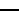
\includegraphics[#1]{rectitude.pdf}}
\newcommand{\planeite}[1][] {
\includegraphics[#1]{planeite.pdf}}
\newcommand{\circularite}[1][] {
\includegraphics[#1]{circularite.pdf}}
\newcommand{\cylindricite}[1][] {
\includegraphics[#1]{cylindricite.pdf}}
\newcommand{\profilLigne}[1][] {
\includegraphics[#1]{profilLigne.pdf}}
\newcommand{\profilSurface}[1][] {
\includegraphics[#1]{profilSurface.pdf}}
\newcommand{\coaxialite}[1][] {
\includegraphics[#1]{coaxialite.pdf}}
\newcommand{\concentricite}[1][] {\coaxialite[#1]}
\newcommand{\symetrie}[1][] {
\includegraphics[#1]{symetrie.pdf}}
\newcommand{\localisation}[1][] {
\includegraphics[#1]{localisation.pdf}}
\newcommand{\parallelisme}[1][] {
\includegraphics[#1]{parallelisme.pdf}}
\newcommand{\perpendicularite}[1][] {
\includegraphics[#1]{perpendicularite.pdf}}
\newcommand{\inclinaison}[1][] {
\includegraphics[#1]{inclinaison.pdf}}
\newcommand{\battementSimple}[1][] {
\includegraphics[#1]{battement.pdf}}
\newcommand{\battement}[1][] {\battementSimple[#1]}
\newcommand{\battementTotal}[1][] {
\includegraphics[#1]{battement_total.pdf}}
%%%%%%%%%%%%%%%%%%%%%%%%%%%%%%%%%%%%%%%%%%%%
%
%	Notation en fabrication
%
%%%%%%%%%%%%%%%%%%%%%%%%%%%%%%%%%%%%%%%%%%%%


%Mouvements de coup
%----------------------------------------
\newcommand{\vCoupe}	{\ensuremath{V_c}}	%Vitesse de coupe
\newcommand{\Vc}	{\vCoupe}		%Vitesse de coupe (raccourci)
\newcommand{\Vavance}	{\ensuremath{V_f}}	%Vitesse d'avance
\newcommand{\Vf}	{\Vavance}		%Vitesse d'avance (raccourci)
\newcommand{\Veco}	{\ensuremath{V_{CE}}}	%Vitesse économique de coupe

\newcommand{\avance}	{\ensuremath{f}}		%Avance de l'outil
\newcommand{\pPasse}	{\ensuremath{a}}	%Profondeur de passe


%Geometrie de l'outil
%--------------------------------

%Angles
\newcommand{\aCoupe}		{\ensuremath{	\gamma	}}		%Angle de coupe
\newcommand{\aDepouille}	{\ensuremath{	\alpha	}}		%Angle de dépouille
\newcommand{\aTaillant}		{\ensuremath{	\beta	}}		%Angle de dépouille
\newcommand{\aInclinaison}	{\ensuremath{	\lambda_r	}}	%Angle d'inclinaison
\newcommand{\aInc}		{\aInclinaison}				%Angle d'inclinaison (raccourci)
\newcommand{\aDirectionArete}	{\ensuremath{	\kappa_r	}}	%Angle de direction d'arete
\newcommand{\aDir}		{\aDirectionArete}			%Angle de direction d'arete (raccourci)
\newcommand{\Kr}		{\aDirectionArete}			%Angle de direction d'arete (raccourci)
\newcommand{\aPointe}		{\ensuremath{	\varepsilon_r	}}			%Angle de direction d'arete (raccourci)

%Plans
\newcommand{\fCoupe}		{\ensuremath{	A_\aCoupe	}}	%Face de coupe
\newcommand{\fDepouille}	{\ensuremath{	A_\aDepouille	}}	%Face de dépouille
\newcommand{\pRef}		{\ensuremath{	P_r	}}		%Plan de référence
\newcommand{\pTravail}		{\ensuremath{	P_f	}}		%Plan de travail conventionnel
\newcommand{\pArete}		{\ensuremath{	P_s	}}		%Plan d'arete de l'outil
\newcommand{\pNormal}		{\ensuremath{	P_n	}}		%Plan d'arete de l'outil

%Autre
\newcommand{\rBec}		{\ensuremath{	R_\varepsilon	}}	%Rayon de bec de l'outil
\newcommand{\usureDepouille}	{\ensuremath{	VB	}}		%Usure en dépouille



%Efforts
%------------------------------------

\newcommand{\FCoupe}		{\ensuremath{	F_c	}}			%Effort de coupe (tangentiel)
\newcommand{\Fc}		{\FCoupe}					%Effort de coupe (tangentiel) (raccourci)
\newcommand{\pSpecifique}	{\ensuremath{	K_c	}}		%Pression specifique de coupe
\newcommand{\Kc}		{\pSpecifique}				%Pression specifique de coupe (raccourci)
\newcommand{\Pcoupe}		{\ensuremath{	P_c	}}		%puissance de coupe
\newcommand{\Pc}		{\Pcoupe}					%puissance de coupe (raccourci)

\newcommand{\cTotal}		{\ensuremath{	C_T	}}		%Cout total
\newcommand{\CT}		{\cTotal}				%Cout total (raccourci)


%Torseur
%=================================================

\newcommand{\tStatique}[2]	{\ensuremath{	\torseur{\T_{\left({#1}\rightarrow{#2}\right)}}	}}


%Résultates
%=================================


\newcommand{\vForce}[3][F]	{\ifthenelse{\equal{#2}{}}
					{\vecteur{{#1}_{#3}}}
					{\vecteur{{#1}_{\left(#2\rightarrow#3\right)}}	}}
\newcommand{\vF}[2][]		{\vForce[F]{#1}{#2}}	%Raccourci
\newcommand{\vT}[2][]		{\vForce[T]{#1}{#2}}	%Raccourci
\newcommand{\vP}[2][]		{\vForce[P]{#1}{#2}}	%Raccourci
\newcommand{\vQ}[2][]		{\vForce[Q]{#1}{#2}}	%Raccourci

%Moments
%==================================

\newcommand{\momentForce}[3]	{\moment[#2\rightarrow#3]{#1}}

%\momentAMnn{P_2}{0}{1}{1}
\newcommand{\momentAMnn}[4]{
\ensuremath{
\vecteur{M}_{#1}^{#4}(#2\to#3)
}
}


\newcommand{\resultanteAMnn}[3]{
\ensuremath{
\vecteur{R}^{#3}(#1\to#2)
}
}

\newcommand{\tActionMecaniqueCann}[9]{\tActionMecaniqueCan{#1}{#2}{#3}{#4}{#5}{#6}{#7}{#8}{#8}}

\newcommand{\momentAM}[3]{
\ensuremath{
\vecteur{M}_{#1}(#2\to#3)
}
}



\newcommand{\resultanteAM}[2]{
\ensuremath{
\vecteur{R}_{#1\to#2}
}
}


%%%%%%%%%%%%%%%%%%%%%%%%%%%%
%
% Notations math�matiques
%
%%%%%%%%%%%%%%%%%%%%%%%%%%%%%%%

\newcommand{\ssi}{si et seulement si }
\newcommand{\indiceGauche}[2]	{\ensuremath{	{\vphantom{#2}}_{#1}{#2} 	}}
\newcommand{\exposantGauche}[2]	{\ensuremath{	{\vphantom{#2}}^{#1}{#2} 	}}
\newcommand{\transposee}[1]	{\ensuremath{	\exposantGauche{\mathit t}{#1}	}}%{\vphantom{#1}}_{\mathit t}{#1}	}}

% FONCTION
%%%%%%%%%%%%%%%%%%%%
\newcommand{\fonction}[2]	{\ensuremath{	{#1}_{\left(#2\right)}		}}
\newcommand{\f}[2]		{	\fonction{#1}{#2}		}
\newcommand{\deriv}[3][]	{\ifthenelse{\equal{#1}{}}	{\ensuremath{	\frac{d{#2}}{d{#3}}}}	{\ensuremath{	\left[\frac{d{#2}}{d{#3}}\right]_{#1}}}}
\newcommand{\atan}[1][]		{\ifthenelse{\equal{#1}{}}	{\ensuremath{	\tan^{-1}	}}	{\ensuremath{	\tan^{-1}\left(#1\right)	}}}


% ENSEMBLES
%%%%%%%%%%%%%%%%%%%%%%%%%%%%%%
\newcommand{\R}		{\ensuremath{\mathbb{R}}	}
\newcommand{\couple}[2]{\ensuremath{\left(#1,#2\right)}}	%Couple (ex : (U,V) )
\newcommand{\triplet}[3]{\ensuremath{\left(#1,#2,#3\right)}}	%Triplet (ex : (U,V,W) )
\newcommand{\quadruplet}[4]{\ensuremath{\left(#1,#2,#3,#4\right)}}	%Triplet (ex : (U,V,W) )



% GEOMETRIE
%%%%%%%%%%%%%%%%%%%%%%%%%%
\newcommand{\segment}[1]	{\ensuremath{	\left[#1\right]		}}		%Fait un sement
\newcommand{\droite}[1]		{\ensuremath{	\left(#1\right)		}}
\newcommand{\arc}[1]		{\ensuremath{	\overset{\frown}{#1}	}}		%Arc
\renewcommand{\angle}[1]	{\ensuremath{	\left(\widehat{#1}\right)	}} %(Red�fini : la fonction angle correspondait au symbole angle)
%%%%%%%%%%%%%%%%%%%%%%%%%%%%%%%%%%%%%%%%%%%
%	unit�s
%%%%%%%%%%%%%%%%%%%%%%%%%%%%%%%%%%%%%%%%%%


\newcommand{\unite}[1]	{{\,\PETIT{\ensuremath{	\color{black}\text{#1}	}}}}

%Longueurs
\newcommand{\mm} 	{\unite{mm}}
\newcommand{\cm} 	{\unite{cm}}
\newcommand{\m} 	{\unite{m}}
\newcommand{\dam} 	{\unite{dam}}
%\newcommand{\hm} 	{\unite{hm}}
\newcommand{\km} 	{\unite{km}}
\newcommand{\orto}{^{\circ}} %degre


%Forces
\newcommand{\N} 	{\unite{N}}
\newcommand{\daN} 	{\unite{daN}}
\newcommand{\Nm} 	{\unite{N\,m}}
\newcommand{\Pa} 	{\unite{Pa}}
\newcommand{\MPa} 	{\unite{MPa}}
\newcommand{\br} 	{\unite{bar}}


%Temps
\renewcommand{\sec} 	{\unite{s}}
\newcommand{\mn} 	{\unite{min}}
\newcommand{\h} 	{\unite{h}}

%Masse
\newcommand{\g} 	{\unite{g}}
\newcommand{\Kg} 	{\unite{Kg}}
%%%%%%%%%%%%%%%%%%%%%%%%%%%%%%%%%%%%%%%%%%%%%
%
%	Notations Analyse fonctionnelle
%
%%%%%%%%%%%%%%%%%%%%%%%%%%%%%%%%%%%%%%%%%%%%


%Analyse fonctionnelle
\newcommand{\MO}	{mati�re d'\oe uvre}
\newcommand{\VA}	{valeur ajout�e}

%%%%%%%%%%%%%%%%%%%%%%%%%%%%%%%%%%%%%%%%%%%%%
%
%	Notations asservissements
%
%%%%%%%%%%%%%%%%%%%%%%%%%%%%%%%%%%%%%%%%%%%%

%Automatique
\newcommand{\TOR}	{		tout-ou-rien	}
\renewcommand{\L}	{\ensuremath{	\mathscr{L}	}}	%Transform�e de Laplace (anciennement un L barr�)
%%%%%%%%%%%%%%%%%%%%%%%%%%%%%%%%%%%%%%%%%%%%%
%
%	Notations vecteurs/torseurs
%
%%%%%%%%%%%%%%%%%%%%%%%%%%%%%%%%%%%%%%%%%%%%



%Commandes de base
%-----------------------------
\newcommand{\vecteur}[1]	{\ensuremath{	\protect\overrightarrow{#1}}}	%Fait un vecteur
\newcommand{\vecteurIndice}[2]	{\ifthenelse{\equal{#2}{\ }}{\vecteur{{#1}}\ }{\vecteur{{#1}_{#2}}}}	%Fait un vecteur avec un indice (x1, y1...), ou un vecteur simple si indice = espace
\newcommand{\vecteurChamp}[2]	{\fonction{\vecteur{#1}}{#2}}
\newcommand{\bipoint}[2]	{\ensuremath{	\vecteur{\segment{#1#2}}	}}	%bipoint
\newcommand{\vLie}[2]		{\ensuremath{	\couple{#1}{#2}	}}			%Vecteur lie
\newcommand{\vGlissant}[2]	{\ensuremath{	\couple{#1}{#2}	}}			%Vecteur glissant
\newcommand{\fN}[2][] {\ensuremath{	\protect\overrightarrow{N_{#1\rightarrow#2}}}}			%Vecteur lie
\newcommand{\fT}[2][]	{\ensuremath{	\protect\overrightarrow{T_{#1\rightarrow#2}}}}
\newcommand{\fpbis}	{\ensuremath{	\protect\overrightarrow{f_{p (S_1\rightarrow S_2)}}}}

%Espaces
%--------------------------------
\newcommand{\eAffine}[1][3]	{\ensuremath{	\mathscr{E}^{#1}	}}	%Espace affine
\newcommand{\eVectoriel}[1][3]	{\ensuremath{	E^{#1}			}}	%Espace vectoriel



%Repr�sentation des vecteurs
\newcommand{\vColonne}[2][]	{\ensuremath{	\left( \begin{array}{c} #2 \end{array} \right)_{#1}	}}	%Vecteur colonne (avec coordonn�es)


%Operateurs Vectoriel

\newcommand{\norme}[1]		{\ensuremath{	\left\Vert #1 \right\Vert	}}	%Norme
\newcommand{\abs}[1]		{\ensuremath{	\left\vert #1 \right\vert	}}	%Valeur absolue
\newcommand{\prodMixte}[3]	{\ensuremath{	\left(#1\wedge#2\right)\cdot#3	}}	%produit mixte
\newcommand{\doubleProdVect}[3]	{\ensuremath{	#1\wedge\left(#2\wedge#3\right)	}}	%produit vectoriel



%VECTEUR PRE-FAVRIQUES
%------------------------------


\newcommand{\vNul}		{\ensuremath{	\overrightarrow{0}	}}	%Symbole d'une base
\newcommand{\vPreFab}[2][]	{\ifthenelse{\equal{#1}{}}	{\vecteur{#2}}	{\vecteurChamp{#2}{#1}}	}	%Vecteur qui choisit tout seul si c'est un vecteur simple ou un champ (pr�sence d'un parametre ou non)


%Tout ce qui est vecteurs e_i
\newcommand{\ve}[1]{\vecteurIndice{e}{#1}}

\newcommand{\vex}{\ve{x}}	%e_x
\newcommand{\vey}{\ve{y}}	%e_y
\newcommand{\vez}{\ve{z}}	%e_z

%\newcommand{\e}{\ensuremath{\overrightarrow {e_2}}}
%\newcommand{\e}{\ensuremath{\overrightarrow {e_3}}}

\newcommand{\vx}[1]{\vecteurIndice{x}{#1}}	%x_i
\newcommand{\vy}[1]{\vecteurIndice{y}{#1}}	%y_i
\newcommand{\vz}[1]{\vecteurIndice{z}{#1}}	%z_i

%\newcommand{\vXzero}{\ensuremath{\vecteur{x_1}}}
%\newcommand{\vYun}{\ensuremath{\vecteur{y_1}}}
%\newcommand{\vZun}{\ensuremath{\vecteur{z_1}}}

%\newcommand{\vXun}{\ensuremath{\vecteur{x_1}}}
%\newcommand{\vYun}{\ensuremath{\vecteur{y_1}}}
%\newcommand{\vZun}{\ensuremath{\vecteur{z_1}}}

%\newcommand{\vXdeux}{\ensuremath{\vecteur{x_2}}}
%\newcommand{\vYdeux}{\ensuremath{\vecteur{y_2}}}
%\newcommand{\vZdeux}{\ensuremath{\vecteur{z_2}}}


\newcommand{\vn}[1][]	{	\vPreFab[#1]{n}	}

\newcommand{\vu}[1][]	{	\vPreFab[#1]{u}	}
\newcommand{\vU}[1][]	{	\vPreFab[#1]{U}	}
%\ifthenelse{\equal{#1}{}}	{\vecteur{U}}	{\vecteurChamp{U}{#1}}	}
%\newcommand{\vU}[1][]	{\ifthenelse{\equal{#1}{}}	{ \ensuremath{\overrightarrow{U}}  }{   \ensuremath{\overrightarrow{U_{(#1)}}}     }}	%Vecteur U ou champ U(M)

\newcommand{\ux}{\ensuremath{u_x}}
\newcommand{\uy}{\ensuremath{u_y}}
\newcommand{\uz}{\ensuremath{u_z}}

\newcommand{\vv}[1][]	{	\vPreFab[#1]{v}	}
\newcommand{\vV}[1][]	{	\vPreFab[#1]{V}	}
%\newcommand{\vV}[1]{\vecteur{V_{#1}}}
%\newcommand{\vV}[1][]{\ifthenelse{\equal{#1}{}}{ \ensuremath{\overrightarrow{V}}  }{   \ensuremath{\overrightarrow{V_{(#1)}}}     }}
%\newcommand{\Vx}{\ensuremath{v_x}}	\newcommand{\vx}{\Vx}
%\newcommand{\Vy}{\ensuremath{v_y}}	\newcommand{\vy}{\Vy}
%\newcommand{\Vz}{\ensuremath{v_z}}	\newcommand{\vz}{\Vz}


\newcommand{\vw}[1][]	{	\vPreFab[#1]{w}	}
\newcommand{\vW}[1][]	{	\vPreFab[#1]{W}	}
%\ifthenelse{\equal{#1}{}}	{\vecteur{W}}	{\vecteurChamp{W}{#1}}	}
%\newcommand{\vW}[1][]{\ifthenelse{\equal{#1}{}}{ \ensuremath{\overrightarrow{W}}  }{   \ensuremath{\overrightarrow{W_{(#1)}}}     }}
\newcommand{\Wx}{\ensuremath{w_x}}	%\newcommand{\wx}{\Wx}
\newcommand{\Wy}{\ensuremath{w_y}}	%\newcommand{\wy}{\Wy}
\newcommand{\Wz}{\ensuremath{w_z}}	%\newcommand{\wz}{\Wz}

\newcommand{\vOM}[1][]	{	\vPreFab[#1]{OM}	}
\newcommand{\OM}[1][]	{	\vOM[#1]	}
\newcommand{\Mx}{\ensuremath{m_x}}	\newcommand{\mx}{\Mx}
\newcommand{\My}{\ensuremath{m_y}}	\newcommand{\my}{\My}
\newcommand{\Mz}{\ensuremath{m_z}}	\newcommand{\mz}{\Mz}

\newcommand{\vUun}{\ensuremath{\vecteur{U_1}}}
\newcommand{\vUn}{\ensuremath{\vecteur{U_n}}}
\newcommand{\vVun}{\ensuremath{\vecteur{U_1}}}
\newcommand{\vVp}{\ensuremath{\vecteur{V_p}}}


\newcommand{\vOP}[1][]	{	\vPreFab[#1]{OP}	}
\newcommand{\OP}[1][]	{	\vOP[#1]	}

\newcommand{\vAB}[1][]	{	\vPreFab[#1]{AB}	}
\newcommand{\AB}[1][]	{	\vAB[#1]	}

\newcommand{\vBA}[1][]	{	\vPreFab[#1]{BA}	}
\newcommand{\BA}[1][]	{	\vBA[#1]	}

\newcommand{\vOA}[1][]	{	\vPreFab[#1]{OA}	}
\newcommand{\OA}[1][]	{	\vOA[#1]	}

\newcommand{\vOB}[1][]	{	\vPreFab[#1]{OB}	}
\newcommand{\OB}[1][]	{	\vOB[#1]	}

\newcommand{\vi}[1]	{\ensuremath{	\vecteur{i_{#1}}	}}
\newcommand{\vj}[1]	{\ensuremath{	\vecteur{j_{#1}}	}}
\newcommand{\vk}[1]	{\ensuremath{	\vecteur{k_{#1}}	}}


%Bases
%-------------------------
\newcommand{\B}		{\ensuremath{	\mathscr{B}	}}	%Symbole d'une base
\newcommand{\Bxyz}	{\triplet{\vex}{\vey}{\vez}}
\newcommand{\Buvw}	{\triplet{\vu}{\vv}{\vw}}
\newcommand{\base}[3]	{\ensuremath{\left(#1,#2,#3\right)}}	


%Repere
%-------------------------
%\newcommand{\repere}[4]	{\ensuremath{	\left(#1,#2,#3,#4\right)	}}

%%%%%%%%%%%%%%%%%%%%%%%%%%%%%%%%%%%%%%%%%%
%
%	NOTATION TORSEURS
%
%%%%%%%%%%%%%%%%%%%%%%%%%%%%%%%%%%%%%%%%%




%Ecriture
%--------------------------------------
\newcommand{\T}			{\ensuremath{	\mathcal{T}			}}	%T en joli
\newcommand{\torseur}[1]	{\ensuremath{	\left\lbrace #1\right\rbrace	}}	%Torseur quelconque
\newcommand{\tT}{\ensuremath{\torseur{\mathcal{T}}}}	%Torseur T
\newcommand{\tNul}{\ensuremath{\torseur{0}}}	%Torseur T

%Elements de reduction
\newcommand{\M}	{\ensuremath{	\mathcal{M}	}}	%M en joli
\newcommand{\resultante}[2][]	{\ifthenelse{\equal{#1}{}}
					{\ensuremath{	\vecteur{R_{\left(#2\right)}}	}}
					{\ensuremath{	\vecteur{R_{\left(#1\rightarrow#2\right)}}	}}}	%\restultante[origine]{ensembleIsole}
\newcommand{\moment}[3][]	{\ifthenelse{\equal{#1}{}}
					{\ensuremath{	\vecteur{{\M_{#2}}_{\left(#3\right)}}	}}
					{\ensuremath{	\vecteur{{\M_{#1}}_{\left(#2\rightarrow#3\right)}}	}}}
\newcommand{\torseurLigne}[3]	{\ensuremath{	\indiceGauche{#1}{\left\lbrace\begin{array}{c}#2\\#3\end{array}\right\rbrace}	}}
\newcommand{\tLigne}[3]		{\ensuremath{	\torseurLigne{#1}{#2}{#3}	}}
\newcommand{\torseurColonne}[4]	{\ensuremath{	\indiceGauche{#1}{\left\lbrace\begin{array}{c}#2\end{array}\begin{array}{c}#3\end{array}\right\rbrace}_{#4}	}}
\newcommand{\tColonne}[4]	{\ensuremath{	\torseurColonne{#1}{#2}{#3}{#4}	}}


%Operateurs
\newcommand{\automoment}[1][\T]{\ensuremath{a_{(#1)}}}




%%%%%%%%%%%%%%%%%%%%%%%%%%%%%%%

%	Cin�matique

%%%%%%%%%%%%%%%%%%%%%%%%%%%%%%%
\RequirePackage{tikz}



%Raccourcis
\newcommand{\CIR}	{centre instantan� de rotation}
\newcommand{\cir}	{\CIR}
\newcommand{\Cir}	{Centre instantan� de rotation}


%DDL
\newcommand{\Rx}	{\ensuremath{	R_x	}}
\newcommand{\Ry}	{\ensuremath{	R_y	}}
\newcommand{\Rz}	{\ensuremath{	R_z	}}

\newcommand{\Tx}	{\ensuremath{	T_x	}}
\newcommand{\Ty}	{\ensuremath{	T_y	}}
\newcommand{\Tz}	{\ensuremath{	T_z	}}



%G�om�trie
\newcommand{\solide}[1]	{\ensuremath{	#1	}}		%Solide
\newcommand{\sS}[1]	{\solide{S_{#1}}}	%Solides S1, S2, ...
\newcommand{\s}[1]	{\ensuremath{(#1)}}	%Solides (1), (2), ...

%Rep�res
\newcommand{\repere}[4]	{\ensuremath{	\left(#1,#2,#3,#4\right)	}}
\newcommand{\rR}[1]	{\ensuremath{	R_{#1}	}	}


%coordonn�es variables fonction du temps
\newcommand{\xt}	{\fonction{x}{t}}
\newcommand{\yt}	{\fonction{y}{t}}
\newcommand{\zt}	{\fonction{z}{t}}
\newcommand{\rt}	{\fonction{r}{t}}
\newcommand{\thetat}	{\fonction{\theta}{t}}

\newcommand{\thetap}	{\ensuremath{\dot\theta}}

\newcommand{\xtp}	{\fonction{\dot{x}}{t}}
\newcommand{\ytp}	{\fonction{\dot{y}}{t}}
\newcommand{\ztp}	{\fonction{\dot{z}}{t}}
\newcommand{\rtp}	{\fonction{\dot{r}}{t}}
\newcommand{\thetatp}	{\fonction{\dot\theta}{t}}

%Vitesse
\newcommand{\vVitesse}[3][]		{\ifthenelse{\equal{#1}{}}{\vecteur{V_{\left(#2/#3\right)}}}{\vecteur{V_{\left(#1\in#2/#3\right)}}}	}%{\vecteurChamp{V}{#2/#3}}{\vecteurChamp{V}{#1\in#2/#3}}}
\newcommand{\vAcceleration}[3][]	{\ifthenelse{\equal{#1}{}}{\vecteur{\Gamma_{#2/#3}}}{\vecteur{\Gamma_{#1\in#2/#3}}}}
\newcommand{\vRotation}[2]		{\vecteur{\Omega_{\left(#1/#2\right)}}}
\newcommand{\vPivotement}[2]		{\vecteur{{\Omega_p}_{\left(#1/#2\right)}}}
\newcommand{\vRoulement}[2]		{\vecteur{{\Omega_r}_{\left(#1/#2\right)}}}

%D�placement de vitesse
\newcommand{\deplaceVitesse}[4]	{\ensuremath{	\vVitesse[#3]{#1}{#2}+\vecteur{#4#3}\wedge\vRotation{#1}{#2}	}}	%\deplaceVitesse{Solid}{Referentiel}{Pdepart}{Parrivee}


%petits d�placements
\newcommand{\vDeplacement}[3][]		{\ifthenelse{\equal{#1}{}}{\vecteur{U_{#2/#3}}}{\vecteur{U_{#1\in#2/#3}}}}
\newcommand{\vDep}[3][]			{\vDeplacement[#1]{#2}{#3}}
\newcommand{\vPetitDeplacement}[3][]	{\ifthenelse{\equal{#1}{}}{\vecteur{U_{#2/#3}}}{\vecteur{U_{#1\in#2/#3}}}}
\newcommand{\vPetitDep}[3][]		{\vPetitDeplacement[#1]{#2}{#3}}
\newcommand{\vPetiteRotation}[2]	{\vecteur{\theta_{#1/#2}}}
\newcommand{\vPetiteRot}[2]		{\vPetiteRotation{#1}{#2}}

\newcommand{\wx}			{\ensuremath{	\omega_x	}}
\newcommand{\wy}			{\ensuremath{	\omega_y	}}
\newcommand{\wz}			{\ensuremath{	\omega_z	}}

%Torseur
\newcommand{\V}				{\ensuremath{	\mathscr{V}	}}	%Symbole du torseur cinematique
\newcommand{\C}				{\ensuremath{	\mathscr{C}	}}	%Symbole du torseur cinetique
\newcommand{\Dyn}				{\ensuremath{	\mathscr{D}	}}	%Symbole du torseur dynamique
\newcommand{\tCinematique}[3][]		{\ensuremath{	\torseur{\V^{#1}_{\left(#2/#3\right)}}	}}%torseur cinematique
\newcommand{\tCinetique}[3][]		{\ensuremath{	\torseur{\C^{#1}_{\left(#2/#3\right)}}	}}%torseur cinetique
\newcommand{\tDynamique}[3][]		{\ensuremath{	\torseur{\Dyn^{#1}_{\left(#2/#3\right)}}	}}%torseur dynamique
\newcommand{\tV}[2]			{\tCinematique{#1}{#2}}	%torseur cinematique
\newcommand{\tC}[2]			{\tCinetique{#1}{#2}}	%torseur cinetique
\newcommand{\tDyn}[2]			{\tDynamique{#1}{#2}}	%torseur dynamique
\newcommand{\D}				{\ensuremath{	\mathscr{D}	}}	%Symbole du torseur petit d�placement
\newcommand{\tPetitDeplacement}[3][]	{\ensuremath{	\torseur{\D^{#1}_{\left(#2/#3\right)}}	}}%torseur petit d�placement
\newcommand{\tPetitDep}[3][]		{\tPetitDeplacement[#1]{#2}{#3}}
\newcommand{\tD}[3][]			{\tPetitDeplacement[#1]{#2}{#3}}

%Moments dynamiques et cinetiques
\newcommand{\vSigma}[3][]		{\ifthenelse{\equal{#1}{}}{\vecteur{\sigma_{\left(#2/#3\right)}}}{\vecteur{\sigma_{#1}\left(#2/#3\right)}}	}%{\vecteurChamp{V}{#2/#3}}{\vecteurChamp{V}{#1\in#2/#3}}}
\newcommand{\vDelta}[3][]		{\ifthenelse{\equal{#1}{}}{\vecteur{\delta_{\left(#2/#3\right)}}}{\vecteur{\delta_{#1}\left(#2/#3\right)}}	}%{\vecteurChamp{V}{#2/#3}}{\vecteurChamp{V}{#1\in#2/#3}}}
%Graphique / figures
%Figures planes de projection
\newcommand{\scFigCalc}[6][]{
\begin{tikzpicture}
\draw[->] (0,0) -- (3,0) node[above] {$\overrightarrow{#2}$};
\draw[->] (0,0) -- (0,3) node[right] {$\overrightarrow{#3}$};
\draw[->] (0cm,0cm) -- (25:3cm) node[above] {$\overrightarrow{#4}$};
\draw[->] (0cm,0cm) -- (115:3cm) node[right] {$\overrightarrow{#5}$};
\draw[->] (1,0) arc (0:25:1cm)node[right=0.5em] {$#6$} ;
\draw[->] (0,1) arc (90:115:1cm)node[above=0.5em] {$#6$} ;
\node[below](0,0){$\overrightarrow{#1}$};
\end{tikzpicture}
}



%%%%%%%%%%%%%%%%%%%%%%%%%%

%NOTATION

%COTATION FONCTIONNELLE

%%%%%%%%%%%%%%%%%%%%%%%%





% Cotes
%%%%%%%%%%%%%%%%%%%%%%%%%%%%%%%%

\newcommand{\dnom}	{\ensuremath{d_{\text{nom}}}}	%Diam�tre nominal
\newcommand{\dmoy}	{\ensuremath{d_{\text{moy}}}}	%Diam�tre nominal
\newcommand{\dinf}	{\ensuremath{d_{\text{inf}}}}	%Diam�tre nominal
\newcommand{\dsup}	{\ensuremath{d_{\text{sup}}}}	%Diam�tre nominal


% Symboles
%%%%%%%%%%%%%%%%%%%%%%%%%%%%%%%%

\newcommand{\rectitude}[1][] {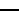
\includegraphics[#1]{rectitude.pdf}}
\newcommand{\planeite}[1][] {
\includegraphics[#1]{planeite.pdf}}
\newcommand{\circularite}[1][] {
\includegraphics[#1]{circularite.pdf}}
\newcommand{\cylindricite}[1][] {
\includegraphics[#1]{cylindricite.pdf}}
\newcommand{\profilLigne}[1][] {
\includegraphics[#1]{profilLigne.pdf}}
\newcommand{\profilSurface}[1][] {
\includegraphics[#1]{profilSurface.pdf}}
\newcommand{\coaxialite}[1][] {
\includegraphics[#1]{coaxialite.pdf}}
\newcommand{\concentricite}[1][] {\coaxialite[#1]}
\newcommand{\symetrie}[1][] {
\includegraphics[#1]{symetrie.pdf}}
\newcommand{\localisation}[1][] {
\includegraphics[#1]{localisation.pdf}}
\newcommand{\parallelisme}[1][] {
\includegraphics[#1]{parallelisme.pdf}}
\newcommand{\perpendicularite}[1][] {
\includegraphics[#1]{perpendicularite.pdf}}
\newcommand{\inclinaison}[1][] {
\includegraphics[#1]{inclinaison.pdf}}
\newcommand{\battementSimple}[1][] {
\includegraphics[#1]{battement.pdf}}
\newcommand{\battement}[1][] {\battementSimple[#1]}
\newcommand{\battementTotal}[1][] {
\includegraphics[#1]{battement_total.pdf}}
%%%%%%%%%%%%%%%%%%%%%%%%%%%%%%%%%%%%%%%%%%%%%
%
%	Notation en fabrication
%
%%%%%%%%%%%%%%%%%%%%%%%%%%%%%%%%%%%%%%%%%%%%


%Mouvements de coup
%----------------------------------------
\newcommand{\vCoupe}	{\ensuremath{V_c}}	%Vitesse de coupe
\newcommand{\Vc}	{\vCoupe}		%Vitesse de coupe (raccourci)
\newcommand{\Vavance}	{\ensuremath{V_f}}	%Vitesse d'avance
\newcommand{\Vf}	{\Vavance}		%Vitesse d'avance (raccourci)
\newcommand{\Veco}	{\ensuremath{V_{CE}}}	%Vitesse économique de coupe

\newcommand{\avance}	{\ensuremath{f}}		%Avance de l'outil
\newcommand{\pPasse}	{\ensuremath{a}}	%Profondeur de passe


%Geometrie de l'outil
%--------------------------------

%Angles
\newcommand{\aCoupe}		{\ensuremath{	\gamma	}}		%Angle de coupe
\newcommand{\aDepouille}	{\ensuremath{	\alpha	}}		%Angle de dépouille
\newcommand{\aTaillant}		{\ensuremath{	\beta	}}		%Angle de dépouille
\newcommand{\aInclinaison}	{\ensuremath{	\lambda_r	}}	%Angle d'inclinaison
\newcommand{\aInc}		{\aInclinaison}				%Angle d'inclinaison (raccourci)
\newcommand{\aDirectionArete}	{\ensuremath{	\kappa_r	}}	%Angle de direction d'arete
\newcommand{\aDir}		{\aDirectionArete}			%Angle de direction d'arete (raccourci)
\newcommand{\Kr}		{\aDirectionArete}			%Angle de direction d'arete (raccourci)
\newcommand{\aPointe}		{\ensuremath{	\varepsilon_r	}}			%Angle de direction d'arete (raccourci)

%Plans
\newcommand{\fCoupe}		{\ensuremath{	A_\aCoupe	}}	%Face de coupe
\newcommand{\fDepouille}	{\ensuremath{	A_\aDepouille	}}	%Face de dépouille
\newcommand{\pRef}		{\ensuremath{	P_r	}}		%Plan de référence
\newcommand{\pTravail}		{\ensuremath{	P_f	}}		%Plan de travail conventionnel
\newcommand{\pArete}		{\ensuremath{	P_s	}}		%Plan d'arete de l'outil
\newcommand{\pNormal}		{\ensuremath{	P_n	}}		%Plan d'arete de l'outil

%Autre
\newcommand{\rBec}		{\ensuremath{	R_\varepsilon	}}	%Rayon de bec de l'outil
\newcommand{\usureDepouille}	{\ensuremath{	VB	}}		%Usure en dépouille



%Efforts
%------------------------------------

\newcommand{\FCoupe}		{\ensuremath{	F_c	}}			%Effort de coupe (tangentiel)
\newcommand{\Fc}		{\FCoupe}					%Effort de coupe (tangentiel) (raccourci)
\newcommand{\pSpecifique}	{\ensuremath{	K_c	}}		%Pression specifique de coupe
\newcommand{\Kc}		{\pSpecifique}				%Pression specifique de coupe (raccourci)
\newcommand{\Pcoupe}		{\ensuremath{	P_c	}}		%puissance de coupe
\newcommand{\Pc}		{\Pcoupe}					%puissance de coupe (raccourci)

\newcommand{\cTotal}		{\ensuremath{	C_T	}}		%Cout total
\newcommand{\CT}		{\cTotal}				%Cout total (raccourci)
%

%Torseur
%=================================================

\newcommand{\tStatique}[2]	{\ensuremath{	\torseur{\T_{\left({#1}\rightarrow{#2}\right)}}	}}


%Résultates
%=================================


\newcommand{\vForce}[3][F]	{\ifthenelse{\equal{#2}{}}
					{\vecteur{{#1}_{#3}}}
					{\vecteur{{#1}_{\left(#2\rightarrow#3\right)}}	}}
\newcommand{\vF}[2][]		{\vForce[F]{#1}{#2}}	%Raccourci
\newcommand{\vT}[2][]		{\vForce[T]{#1}{#2}}	%Raccourci
\newcommand{\vP}[2][]		{\vForce[P]{#1}{#2}}	%Raccourci
\newcommand{\vQ}[2][]		{\vForce[Q]{#1}{#2}}	%Raccourci

%Moments
%==================================

\newcommand{\momentForce}[3]	{\moment[#2\rightarrow#3]{#1}}

%\momentAMnn{P_2}{0}{1}{1}
\newcommand{\momentAMnn}[4]{
\ensuremath{
\vecteur{M}_{#1}^{#4}(#2\to#3)
}
}


\newcommand{\resultanteAMnn}[3]{
\ensuremath{
\vecteur{R}^{#3}(#1\to#2)
}
}

\newcommand{\tActionMecaniqueCann}[9]{\tActionMecaniqueCan{#1}{#2}{#3}{#4}{#5}{#6}{#7}{#8}{#8}}

\newcommand{\momentAM}[3]{
\ensuremath{
\vecteur{M}_{#1}(#2\to#3)
}
}



\newcommand{\resultanteAM}[2]{
\ensuremath{
\vecteur{R}_{#1\to#2}
}
}




% BOITES
%%%%%%%%%%%%%%%%%%%%%%%%%%�
%%%%%%%%%%%%%%%%%%%%%%%%%%%%%%%%%%%%%%%%%%
%
%	BOITES
%
%%%%%%%%%%%%%%%%%%%%%%%%%%%%%%%%%%%%%%%%%%



% Environnements
%==================================

\newcommand{\tailleDesBoites}{0.9}%pourcentage de la taille de la ligne





%%%%%%%%%%%%%%%%%%%%%%%%%%%%%%%%%%%%%%%%%%
% DEFINITION
%%%%%%%%%%%%%%%%%%%%%%%%%%%%%%%%%%%%%%%%%%

\definecolor{fond_definition}{RGB}{255,255,255}
\definecolor{bord_definition}{RGB}{0,0,0} 

\newcounter{cptDefinition}	%Compteur de definitions

\newenvironment{definition}[1][]	{\refstepcounter{cptDefinition}
					\begin{center}
						\begin{minipage}{\tailleDesBoites\linewidth}
							\begin{bclogo}[couleur=fond_definition,couleurBord=bord_definition,arrondi=0.2,logo=\bcplume]{Définition \thecptDefinition\ : \emph{#1}}}
					{		\end{bclogo}
						\end{minipage}
					\end{center}}
					
					\newenvironment{definition_large}[1][]	{\refstepcounter{cptDefinition}
					\begin{center}
						\begin{minipage}{1.05\linewidth}
							\begin{bclogo}[couleur=fond_definition,couleurBord=bord_definition,arrondi=0.2,logo=\bcplume]{Définition \thecptDefinition\ : \emph{#1}}}
					{		\end{bclogo}
						\end{minipage}
					\end{center}}



%%%%%%%%%%%%%%%%%%%%%%%%%%%%%%%%%%%%%%%%%%
% partieds
%%%%%%%%%%%%%%%%%%%%%%%%%%%%%%%%%%%%%%%%%%



\newcounter{cptpartieDS}	%Compteur des algorithmes

\newenvironment{partieDS}[1][]	{\refstepcounter{cptpartieDS}
\textbf{Partie \thecptpartieDS\ : \emph{#1}}}


\newenvironment{partieDSst}[1][]	{
\textbf{\emph{#1}}}
					

%%%%%%%%%%%%%%%%%%%%%%%%%%%%%%%%%%%%%%%%%%
% ALGORITHME
%%%%%%%%%%%%%%%%%%%%%%%%%%%%%%%%%%%%%%%%%%



\newcounter{cptAlgorithme}	%Compteur des algorithmes

\newenvironment{algorithme}[1][]	{\refstepcounter{cptAlgorithme}
					\begin{center}
						\begin{minipage}{\tailleDesBoites\linewidth}
							\begin{bclogo}[couleur=fond_definition,couleurBord=bord_definition,arrondi=0.2,logo=\bccrayon]{Algorithme \thecptAlgorithme\ : \emph{#1}}}
					{		\end{bclogo}
						\end{minipage}
					\end{center}}


%%%%%%%%%%%%%%%%%%%%%%%%%%%%%%%%%%%%%%%%%%
% regle
%%%%%%%%%%%%%%%%%%%%%%%%%%%%%%%%%%%%%%%%%%

\definecolor{fond_definition}{RGB}{255,255,255}
\definecolor{bord_definition}{RGB}{0,0,0} 

\newcounter{cptRegle}	%Compteur de definitions

\newenvironment{regle}[1][]	{\refstepcounter{cptRegle}
					\begin{center}
						\begin{minipage}{\tailleDesBoites\linewidth}
							\begin{bclogo}[couleur=fond_definition,couleurBord=bord_definition,arrondi=0.2,logo=\bcplume]{Règle \thecptRegle\ : \emph{#1}}}
					{		\end{bclogo}
						\end{minipage}
					\end{center}}

%------------------
%Programme de colle
%------------------
\newenvironment{programmecolle}[1][]	{
					\begin{center}
						\begin{minipage}{\tailleDesBoites\linewidth}
							\begin{bclogo}[couleur=fond_definition,couleurBord=bord_definition,arrondi=0.2,logo=\bccalendrier]{Programme de colle : \emph{#1}}}
					{		\end{bclogo}
						\end{minipage}
					\end{center}}


%------------------
%Rappels
%------------------
\newenvironment{rappel}[1][]	{
					\begin{center}
						\begin{minipage}{\tailleDesBoites\linewidth}
							\begin{bclogo}[couleur=fond_definition,couleurBord=bord_definition,arrondi=0.2,logo=\bccalendrier]{Rappels : \emph{#1}}}
					{		\end{bclogo}
						\end{minipage}
					\end{center}}
					
%%%%%%%%%%%%%%%%%%%%%%%%%%%%%%%%%%%%%%%%%%
% Bilan
%%%%%%%%%%%%%%%%%%%%%%%%%%%%%%%%%%%%%%%%%%

%\definecolor{fond_bilan}{RGB}{255,255,255}
%\definecolor{bord_bilan}{RGB}{0,0,0} 
%
%\newcounter{cptbilan}	%Compteur de bilan
%
%\newenvironment{bilan}[1][]	{\refstepcounter{cptbilan}
%					\begin{center}
%						\begin{minipage}{\tailleDesBoites\linewidth}
%							\begin{bclogo}[couleur=fond_bilan,couleurBord=bord_bilan,arrondi=0.2,logo=\bccalendrier]{Bilan \thecptbilan\ : \emph{#1}}}
%					{		\end{bclogo}
%						\end{minipage}
%					\end{center}}

\newenvironment{bilan}[1][]	{
					\begin{center}
						\begin{minipage}{\tailleDesBoites\linewidth}
							\begin{bclogo}[couleur=fond_definition,couleurBord=bord_definition,arrondi=0.2,logo=\bccalendrier]{Bilan : \emph{#1}}}
					{		\end{bclogo}
						\end{minipage}
					\end{center}}




%%%%%%%%%%%%%%%%%%%%%%%%%%%%%%%%%%%%%%%%%%
% PRINCIPE
%%%%%%%%%%%%%%%%%%%%%%%%%%%%%%%%%%%%%%%%%%

\definecolor{fond_principe}{RGB}{255,255,255}
\definecolor{bord_principe}{RGB}{0,0,0} 

\newenvironment{principe}[1][]	{	\begin{center}
						\begin{minipage}{\tailleDesBoites\linewidth}
							\begin{bclogo}[couleur=fond_principe,couleurBord=bord_principe,arrondi=0.2,logo=\bcplume]{Principe : \emph{#1}}}
					{		\end{bclogo}
						\end{minipage}
					\end{center}}






%%%%%%%%%%%%%%%%%%%%%%%%%%%%%%%%%%%%%%%%%%
% Remarques
%%%%%%%%%%%%%%%%%%%%%%%%%%%%%%%%%%%%%%%%%%

\definecolor{fond_remarque}{RGB}{255,255,255}%{245,245,255} %Couleur du fond
\definecolor{bord_remarque}{RGB}{200,200,200}

\newcounter{cptRemarque}	%Compteur de remarques

\newenvironment{remarque}[1][]	{\refstepcounter{cptRemarque}	%Incremente le compteur
					\begin{center}
						\begin{minipage}{\tailleDesBoites\linewidth}
							\begin{bclogo}[couleur=fond_remarque,couleurBord=bord_remarque,arrondi=0.2,logo=\bcinfo]{Remarque \thecptRemarque\ : \emph{#1}}}
				{			\end{bclogo}
						\end{minipage}
					\end{center}}

\newenvironment{remarques}[1][]	{\refstepcounter{cptRemarque}
					\begin{center}
						\begin{minipage}{\tailleDesBoites\linewidth}
							\begin{bclogo}[couleur=fond_remarque,couleurBord=bord_remarque,arrondi=0.2,logo=\bcinfo]{Remarques \thecptRemarque\ :\emph{#1}}
								\begin{itemize}}
				{				\end{itemize}
							\end{bclogo}
						\end{minipage}
					\end{center}}





%%%%%%%%%%%%%%%%%%%%%%%%%%%%%%%%%%%%%%%%%%
% Attention
%%%%%%%%%%%%%%%%%%%%%%%%%%%%%%%%%%%%%%%%%%

\definecolor{fond_attention}{RGB}{255,255,255}%{255,240,240} 
\definecolor{bord_attention}{RGB}{255,200,200}%{255,240,240} 

\newenvironment{attention}[1][]	{\begin{center}
					\begin{minipage}{\tailleDesBoites\linewidth}
						\begin{bclogo}[couleur=fond_attention,couleurBord=bord_attention,arrondi=0.2,logo=\bcattention]{Attention : \emph{#1}}}
				{		\end{bclogo}
					\end{minipage}
				\end{center}}





%%%%%%%%%%%%%%%%%%%%%%%%%%%%%%%%%%%%%%%%%%
% IMPORTANT
%%%%%%%%%%%%%%%%%%%%%%%%%%%%%%%%%%%%%%%%%%

\definecolor{fond_important}{RGB}{255,255,255}%{255,240,240} 
\definecolor{bord_important}{RGB}{255,200,200}%{255,240,240} 

\newenvironment{important}[1][]	{\begin{center}
					\begin{minipage}{\tailleDesBoites\linewidth}
						\begin{bclogo}[couleur=fond_important,couleurBord=bord_important,arrondi=0.2,logo=\bcattention]{Important : \emph{#1}}}
				{		\end{bclogo}
					\end{minipage}
				\end{center}}





%%%%%%%%%%%%%%%%%%%%%%%%%%%%%%%%%%%%%%%%%%
% IMPORTANT
%%%%%%%%%%%%%%%%%%%%%%%%%%%%%%%%%%%%%%%%%%

\definecolor{fond_important}{RGB}{255,255,255}%{255,240,240} 
\definecolor{bord_important}{RGB}{255,200,200}%{255,240,240} 

\newenvironment{conclusion}[1][]	{\begin{center}
					\begin{minipage}{\tailleDesBoites\linewidth}
						\begin{bclogo}[couleur=fond_important,couleurBord=bord_important,arrondi=0.2,logo=\bcloupe]{Conclusion : \emph{#1}}}
				{		\end{bclogo}
					\end{minipage}
				\end{center}}

%%%%%%%%%%%%%%%%%%%%%%%%%%%%%%%%%%%%%%%%%%
% PROPRIETES
%%%%%%%%%%%%%%%%%%%%%%%%%%%%%%%%%%%%%%%%%%

\definecolor{bord_propriete}{RGB}{200,200,200}
\definecolor{fond_propriete}{RGB} {255,255,255}

\newcounter{cptPropriete}

\newenvironment{propriete}[1][]	{\refstepcounter{cptPropriete}
				\begin{center}
					\begin{minipage}{\tailleDesBoites\linewidth}
						\begin{bclogo}[couleur=fond_propriete,couleurBord=bord_propriete,arrondi=0.2,logo=\bccrayon]{Propriété \thecptPropriete\ : \emph{#1}}}
				{		\end{bclogo}
					\end{minipage}
				\end{center}}

\newenvironment{proprietes}[1][]{\refstepcounter{cptPropriete}
				\begin{center}
					\begin{minipage}{\tailleDesBoites\linewidth}
						\begin{bclogo}[couleur=fond_propriete,couleurBord=bord_propriete,arrondi=0.2,logo=\bccrayon]{Propriétés \thecptPropriete\ : \emph{#1}}
							\begin{itemize}}
				{			\end{itemize}
						\end{bclogo}
					\end{minipage}
				\end{center}}



%%%%%%%%%%%%%%%%%%%%%%%%%%%%%%%%%%%%%%%%%%
% THEOREME
%%%%%%%%%%%%%%%%%%%%%%%%%%%%%%%%%%%%%%%%%%

\definecolor{bord_theoreme}{RGB}{200,200,200}
\definecolor{fond_theoreme}{RGB} {255,255,255}

\newcounter{cptTheoreme}

\newenvironment{theoreme}[1][]	{\refstepcounter{cptTheoreme}
				\begin{center}
					\begin{minipage}{\tailleDesBoites\linewidth}
						\begin{bclogo}[couleur=fond_theoreme,couleurBord=bord_theoreme,arrondi=0.2,logo=\bccrayon]{Théorème \thecptTheoreme\ : \emph{#1}}}
				{		\end{bclogo}
					\end{minipage}
				\end{center}}
\newenvironment{theoremes}[1][]	{\refstepcounter{cptTheoreme}
				\begin{center}
					\begin{minipage}{\tailleDesBoites\linewidth}
						\begin{bclogo}[couleur=fond_theoreme,couleurBord=bord_theoreme,arrondi=0.2,logo=\bccrayon]{Th�or�mes \thecptTheoreme\ : \emph{#1}}
							\begin{itemize}}
				{			\end{itemize}
						\end{bclogo}
					\end{minipage}
				\end{center}}




%%%%%%%%%%%%%%%%%%%%%%%%%%%%%%%%%%%%%%%%%%
% EXEMPLES
%%%%%%%%%%%%%%%%%%%%%%%%%%%%%%%%%%%%%%%%%%

\definecolor{fond_exemple}{RGB}{255,255,255} %Couleur du fond
\definecolor{bord_exemple}{RGB}{0,0,0} %Couleur du fond

\newcounter{cptExemple}

\newenvironment{exemple}[1][]	{\refstepcounter{cptExemple}
				\begin{center}
					\begin{minipage}{0.95\linewidth}
						\begin{bclogo}[couleur=fond_exemple,couleurBord=bord_exemple,arrondi=0.2,logo=\bcbook]{Exemple \thecptExemple\ : \emph{#1}}}
				{		\end{bclogo}
					\end{minipage}
				\end{center}}

\newenvironment{exemples}[1][]	{\refstepcounter{cptExemple}
				\begin{center}
					\begin{minipage}{0.95\linewidth}
						\begin{bclogo}[couleur=fond_exemple,couleurBord=bord_exemple,arrondi=0.2,logo=\bcbook]{Exemples \thecptExemple\ : \emph{#1}}
							\begin{itemize}}
				{			\end{itemize}
						\end{bclogo}
					\end{minipage}
				\end{center}}
				
\newenvironment{exemple_large}[1][]	{\refstepcounter{cptExemple}
				\begin{center}
					\begin{minipage}{1.05\linewidth}
						\begin{bclogo}[couleur=fond_exemple,couleurBord=bord_exemple,arrondi=0.2,logo=\bcbook]{Exemple \thecptExemple\ : \emph{#1}}}
				{		\end{bclogo}
					\end{minipage}
				\end{center}}				
				
%%%%%%%%%%%%%%%%%%%%%%%%%%%%%%%%%%%%%%%%%%
% DOCUMENTS REPONSES EN TD
%%%%%%%%%%%%%%%%%%%%%%%%%%%%%%%%%%%%%%%%%%

\definecolor{fond_docreponsetd}{RGB}{255,255,255} %Couleur du fond
\definecolor{bord_docreponsetd}{RGB}{0,0,0} %Couleur du fond

\newcounter{cptdocreponsetd}

\newenvironment{docreponsetd}[1][]	{\refstepcounter{cptdocreponsetd}
				\begin{center}
					\begin{minipage}{0.95\linewidth}
						\begin{bclogo}[couleur=fond_docreponsetd,couleurBord=bord_docreponsetd,arrondi=0.2,logo=\bcquestion]{Document réponse \thecptdocreponsetd\ : \emph{#1}}}
				{		\end{bclogo}
					\end{minipage}
				\end{center}}
				
%%%%%%%%%%%%%%%%%%%%%%%%%%%%%%%%%%%%%%%%%%
% REPONSES AUX QUESTIONS EN TD
%%%%%%%%%%%%%%%%%%%%%%%%%%%%%%%%%%%%%%%%%%


\newenvironment{reponsetd}[1][]	{\begin{center}
					\begin{minipage}{0.95\linewidth}
						\begin{bclogo}[couleur=fond_docreponsetd,couleurBord=bord_docreponsetd,arrondi=0.2,logo=\bcoeil]{Réponses aux différentes questions}}
				{		\end{bclogo}
					\end{minipage}
				\end{center}}




%%%%%%%%%%%%%%%%%%%%%%%%%%%%%%%%%%%%%%%%%%
% ASTUCE
%%%%%%%%%%%%%%%%%%%%%%%%%%%%%%%%%%%%%%%%%%

\definecolor{fond_astuce}{RGB}{255,255,255}%{250,250,250} %Couleur du fond
\definecolor{bord_astuce}{RGB}{0,0,0}%{250,250,250} %Couleur du fond

\newcounter{cptAstuce}

\newenvironment{astuce}[1][]	{\refstepcounter{cptAstuce}
				\begin{center}
					\begin{minipage}{0.95\linewidth}
						\begin{bclogo}[couleur=fond_exemple,couleurBord=bord_astuce,arrondi=0.2,logo=\bclampe]{Astuce \thecptAstuce\ : \emph{#1}}}
				{		\end{bclogo}
					\end{minipage}
				\end{center}}

\newenvironment{astuce*}[1][]	{\begin{center}
					\begin{minipage}{0.95\linewidth}
						\begin{bclogo}[couleur=fond_exemple,couleurBord=bord_astuce,arrondi=0.2,logo=\bclampe]{Astuce : \emph{#1}}}
				{		\end{bclogo}
					\end{minipage}
				\end{center}}

\newenvironment{astuces}[1][]	{\refstepcounter{cptAstuce}
				\begin{center}
					\begin{minipage}{0.95\linewidth}
						\begin{bclogo}[couleur=fond_exemple,couleurBord=bord_astuce,arrondi=0.2,logo=\bclampe]{Astuces \thecptAstuce\ : \emph{#1}}
							\begin{itemize}}
				{			\end{itemize}
						\end{bclogo}
					\end{minipage}
				\end{center}}

\newenvironment{astuces*}[1][]	{\begin{center}
					\begin{minipage}{0.95\linewidth}
						\begin{bclogo}[couleur=fond_exemple,couleurBord=bord_astuce,arrondi=0.2,logo=\bclampe]{Astuces : \emph{#1}}
							\begin{itemize}}
				{			\end{itemize}
						\end{bclogo}
					\end{minipage}
				\end{center}}


%%%%%%%%%%%%%%%%%%%%%%%%%%%%%%%%%%%%%%%%%%
% DEMONSTRATION
%%%%%%%%%%%%%%%%%%%%%%%%%%%%%%%%%%%%%%%%%%

\definecolor{fond_demo}{RGB}{255,255,255}%{250,250,250} %Couleur du fond
\definecolor{bord_demo}{RGB}{0,0,0}%{250,250,250} %Couleur du fond

\newcounter{cptDemonstration}

\newenvironment{demonstration}[1][]	{\stepcounter{cptDemonstration}
					\begin{center}
						\begin{minipage}{0.95\linewidth}
							\begin{bclogo}[couleur=fond_demo,couleurBord=bord_demo,arrondi=0.2,logo=\bcpanchant]{Démonstration \thecptDemonstration\ : \emph{#1}}}
					{		\end{bclogo}
						\end{minipage}
					\end{center}}






%%%%%%%%%%%%%%%%%%%%%%%%%%%%%%%%%%%%%%%%%%
% RESUME
%%%%%%%%%%%%%%%%%%%%%%%%%%%%%%%%%%%%%%%%%%

\definecolor{fond_resume}{RGB}{255,255,255}%{250,250,250} %Couleur du fond
\definecolor{bord_resume}{RGB}{0,0,0}%{250,250,250} %Couleur du fond

\newcounter{cptResume}

\newenvironment{resume}[1][]	{\stepcounter{cptResume}
					\begin{center}
						\begin{minipage}{0.95\linewidth}
							\begin{bclogo}[couleur=fond_resume,couleurBord=bord_resume,arrondi=0.2,logo=\bcpanchant]{R�sum� \thecptResume\ : \emph{#1}}}
					{		\end{bclogo}
						\end{minipage}
					\end{center}}

\newenvironment{resume*}[1][]	{	\begin{center}
						\begin{minipage}{0.95\linewidth}
							\begin{bclogo}[couleur=fond_resume,couleurBord=bord_resume,arrondi=0.2,logo=\bcpanchant]{Résumé : \emph{#1}}}
					{		\end{bclogo}
						\end{minipage}
					\end{center}}


%%%%%%%%%%%%%%%%%%%%%%%%%%%%%%%%%%%%%%%%%%
% MAKING-OF
%%%%%%%%%%%%%%%%%%%%%%%%%%%%%%%%%%%%%%%%%%
%MakingOf

%Booleen qui affiche les notes - commentaires
\newboolean{makingOf}
%\setboolean{makingOf}{false}	%Petite condition qui choisit entre 2 formats d'image
\newcommand{\setMakingOfOn}{\setboolean{makingOf}{true}}	%Active le texte � trous
\newcommand{\setMakingOfOff}{\setboolean{makingOf}{false}}	%Active le texte � trous
\setMakingOfOff

\definecolor{fond_makingOf}{RGB}{255,255,255} %Couleur du fond
\definecolor{bord_makingOf}{RGB}{0,0,0} %Couleur du bord

\newenvironment{makingOf}	{
					\setbox0=\vbox\bgroup
				}
				{
					\egroup
					\ifthenelse{\boolean{makingOf}}
						{
							\begin{bclogo}[couleur=fond_makingOf,couleurBord=bord_makingOf,arrondi=0.2,logo=\bcetoile]{Commentaire :}
								\box0
							\end{bclogo}
						}
						{
						}
				}
%\newenvironment{makingOf}{\begin{center}\begin{minipage}{\linewidth}\begin{bclogo}[couleur=fond_makingOf,couleurBord=black,arrondi=0.2,logo=\bcetoile]{Commentaire :}}{\end{bclogo}\end{minipage}\end{center}}

%Zone a trou (l'argument est l'espace vertical que doit prendre le trou)


%%%%%%%%%%%%%%%%%%%%%%%%%%%%%%%%%%%%%%%%%%
% TEXTE CACHE - TROU
%%%%%%%%%%%%%%%%%%%%%%%%%%%%%%%%%%%%%%%%%%
%\newbox\dada
\definecolor{couleurCache}{rgb}{0,0.5,0}
\newenvironment{texteCache}[1][0cm]	{\par
						\ifthenelse{\boolean{texteATrou}}
							{\vspace{#1}\vspace{1.cm}}
							{}
							{}
						\setbox1=\vbox
						\bgroup
					}
					{	\egroup
						\ifthenelse{\boolean{texteATrou}}
							{	\ifthenelse{\boolean{makingOf}}
									{\textcolor{couleurTrou}{\box1}}
									{\phantom{\box1}}%{\vphantom{\box1}}
							}
							{\box1}
						\par
					}
					
\newenvironment{texteCache_DS}[1][0cm]	{\par
						\ifthenelse{\boolean{texteATrou}}
							{\vspace{#1}}
							{}
							{}
						\setbox1=\vbox
						\bgroup
					}
					{	\egroup
						\ifthenelse{\boolean{texteATrou}}
							{	\ifthenelse{\boolean{makingOf}}
									{\textcolor{couleurTrou}{\box1}}
									{\phantom{\box1}}%{\vphantom{\box1}}
							}
							{\box1}
						\par
					}
					
\newenvironment{texteCache_DS_sans_espace}[1][0cm]	{\par
						\ifthenelse{\boolean{texteATrou}}
							{\vspace{#1}}
							{}
							{}
						\setbox1=\vbox
						\bgroup
					}
					{	\egroup
						\ifthenelse{\boolean{texteATrou}}
							{	\ifthenelse{\boolean{makingOf}}
									{\textcolor{couleurTrou}{\box1}}
									{\phantom{\box1}}%{\vphantom{\box1}}
							}
							{\box1}
						\par
					}
%\newenvironment{textCache}[1][0cm]{\setbox\dada=\vbox{\vspace{#1}} \setbox1=\vbox\bgroup}{\egroup\ifthenelse{\boolean{textATrou}}{\box\dada}{\box1}}
%\newenvironment{texteCache}{\setbox1=\hbox\bgroup}{\egroup\ifthenelse{\boolean{textATrou}}{secret}{\box1}}



\newcommand{\remplaceCache}[2]	{\ifthenelse{\boolean{texteATrou} \AND \NOT \boolean{makingOf}}{#1}{#2}}








%%%%%%%%%%%%%%%%%%%%%%%%%%%%%%%%%%%%%%%%%%
% OBJECTIF
%%%%%%%%%%%%%%%%%%%%%%%%%%%%%%%%%%%%%%%%%%

\definecolor{fond_objectif}{RGB}{255,255,255}%{250,250,250} %Couleur du fond
\definecolor{bord_objectif}{RGB}{0,0,0}%{250,250,250} %Couleur du fond

\newcounter{cptObjectif}

\newenvironment{objectif}[1][]	{\refstepcounter{cptObjectif}
				\begin{center}
					\begin{minipage}{0.95\linewidth}
						\begin{bclogo}[couleur=fond_objectif,couleurBord=bord_objectif,arrondi=0.2,logo=\bclampe]{Objectif \thecptObjectif\ : \emph{#1}}}
				{		\end{bclogo}
					\end{minipage}
				\end{center}}
				
				
				\newenvironment{obj}[1][]	{\refstepcounter{cptObjectif}
				\begin{center}
					\begin{minipage}{0.95\linewidth}
						\begin{bclogo}[couleur=fond_objectif,couleurBord=bord_objectif,arrondi=0.2,logo=\bclampe]{Objectif \thecptObjectif\ : \emph{#1}}}
				{		\end{bclogo}
					\end{minipage}
				\end{center}}

\newenvironment{objectif*}[1][]	{\begin{center}
					\begin{minipage}{0.95\linewidth}
						\begin{bclogo}[couleur=fond_objectif,couleurBord=bord_objectif,arrondi=0.2,logo=\bclampe]{Objectif : \emph{#1}}}
				{		\end{bclogo}
					\end{minipage}
				\end{center}}

\newenvironment{objectifs}[1][]	{\refstepcounter{cptObjectif}
				\begin{center}
					\begin{minipage}{0.95\linewidth}
						\begin{bclogo}[couleur=fond_objectif,couleurBord=bord_objectif,arrondi=0.2,logo=\bclampe]{Objectifs \thecptObjectif\ : \emph{#1}}
							\begin{itemize}}
				{			\end{itemize}
						\end{bclogo}
					\end{minipage}
				\end{center}}

\newenvironment{objectifs*}[1][]{\begin{center}
					\begin{minipage}{0.95\linewidth}
						\begin{bclogo}[couleur=fond_objectif,couleurBord=bord_objectif,arrondi=0.2,logo=\bclampe]{Objectifs : \emph{#1}}
							\begin{itemize}}
				{			\end{itemize}
						\end{bclogo}
					\end{minipage}
				\end{center}}







%%%%%%%%%%%%%%%%%%%%%%%%%%%%%%%%%%%%%%%%%%
% EXERCICE
%%%%%%%%%%%%%%%%%%%%%%%%%%%%%%%%%%%%%%%%%%

\newcounter{cptExos}
\newcommand{\exercice}[1]	{\refstepcounter{cptExos}
				\section*{Exercice \thecptExos\ : #1}
				\resetQuestions}
%





%%%%%%%%%%%%%%%%%%%%%%%%%%%%%%%%%%%%%%%%%%
% QUESTION
%%%%%%%%%%%%%%%%%%%%%%%%%%%%%%%%%%%%%%%%%%

\newcounter{cptQuestions}

\newcommand{\resetQuestions}{\setcounter{cptQuestions}{0}}


%\newcommand{\question}[1]
%				{	\par	%Fini un paragraphe
%					\refstepcounter{cptQuestions}
%					%\global\advance\cptQuestions\@ne	%Incr�mente le compteur
%					\vspace{0.3cm}
%					\fbox{\gras{Q\thecptQuestions.}} 
%					{\itshape #1 }
%					%\par\vspace{0.3cm}
%				}

\newcounter{thequestion}
\newcommand{\question}[1]{{\stepcounter{thequestion}\bf Q \arabic{thequestion} : #1}

}

\newcounter{activite}
\newcommand{\activite}[1]{{\stepcounter{activite}\bf Activité \arabic{activite} : #1}

}

%\newenvironment{question}[1][]	{	\par	%Fini un paragraphe
%					\refstepcounter{cptQuestions}
%					%\global\advance\cptQuestions\@ne	%Incr�mente le compteur
%					\itshape\vspace{0.3cm}
%					\fbox{Q\thecptQuestions.} 
%				}
%				{
%					\par\vspace{0.3cm}
%				}


\newenvironment{questions}[1][]	{

					\itshape \vspace{0.3cm}
					\addtocounter{cptQuestions}{-1}	%D�sincr�menter le compteur
					%\global\advance\cptQuestions-\@ne
					%\def\labelitemi{\global\advance\cptQuestions\@ne Q\the\cptQuestions.}
					\renewcommand{\labelitemi}{\refstepcounter{cptQuestions}\fbox{Q\thecptQuestions.}}
					\begin{itemize}
				}
				{
					\end{itemize}\vspace{0.3cm}
				}

\newenvironment{question*}[1][]	{	\par	%Fini un paragraphe
					\itshape\vspace{0.3cm}
					\fbox{Q.} 
				}
				{
					\par\vspace{0.3cm}
				}


\newenvironment{questions*}[1][]	{

					\itshape \vspace{0.3cm}
					\renewcommand{\labelitemi}{\fbox{Q.}}
					\begin{itemize}
				}
				{
					\end{itemize}\vspace{0.3cm}
				}







%%%%%%%%%%%%%%%%%%%%%%%%%%%%%%%%%%%%%%%%%%
% REPONSE
%%%%%%%%%%%%%%%%%%%%%%%%%%%%%%%%%%%%%%%%%%

\newboolean{reponses}
\newcommand{\setReponsesOn}{\setboolean{reponses}{true}}	%Active le texte � trous
\newcommand{\setReponsesOff}{\setboolean{reponses}{false}}	%Active le texte � trous
\setReponsesOff

\newenvironment{reponse}[1][]	{	\par	%Fini un paragraphe
					\setbox1=\vbox
					\bgroup
				}
				{	\egroup
					\ifthenelse{\boolean{makingOf}}
						{\color{red}\box1}
						{	\ifthenelse{\boolean{reponses}}
								{\box1}
								{}
						}
					\par
				}







%%%%%%%%%%%%%%%%%%%%%%%%%%%%%%%%%%%%%%%%%%
% DOCUMENT RESSOURCE
%%%%%%%%%%%%%%%%%%%%%%%%%%%%%%%%%%%%%%%%%%


\newcounter{cptDocRessource}

\newenvironment{docRessource}[1][]
				{	\renewcommand{\thecptDocRessource}{DOC-\arabic{cptDocRessource}}
					\refstepcounter{cptDocRessource}
					\clearpage
					\newpage %Nouvelle page
					\appendix
					
					
					\fbox{\GRAND{\thecptDocRessource}}
				}
				{	
					\clearpage
					\newpage
				}

%%%%%%%%%%%%%%%%%%%%%%%%%%%%%%%%%%%%%%%%%%
% DOCUMENT REPONSE
%%%%%%%%%%%%%%%%%%%%%%%%%%%%%%%%%%%%%%%%%%


\newcounter{cptDocReponse}

\newenvironment{docReponse}[1][]
				{	\renewcommand{\thecptDocReponse}{DR-\arabic{cptDocReponse}}
					\refstepcounter{cptDocReponse}
					\clearpage
					\newpage %Nouvelle page
					
					\begin{tabular}{cc}
						\begin{minipage}{0.5\linewidth}
							\fbox{\GRAND{\thecptDocReponse}}
						\end{minipage}
					&
						\begin{minipage}{0.5\linewidth}
							\begin{flushright}\fbox{\GRAND{Nom : \hspace{6cm}}}\end{flushright}
							                                                   
						\end{minipage}
					\end{tabular}

					
				}
				{
					\clearpage
					\newpage
				}
				
				
				%%% Boîtes pour les documents
\newtcolorbox[auto counter]{pabox}[2][]{%
%sharp corners,boxrule = 0.2mm,colback=white,colbacktitle=white!99!black,colframe=white!5!black,coltitle=black,fonttitle=\bfseries,breakable,
sharp corners,boxrule = 0.2mm,left=1mm,right=1mm,colback=white,colbacktitle=white,colframe=white!5!black,coltitle=black,fonttitle=\bfseries,breakable,
title=Document ~\thetcbcounter~- #2,#1}
\newcommand{\doc}[3]{\begin{pabox}[label={#1}]{#2}#3\end{pabox}}



 \newcounter{exo}


\makeatletter             
\renewcommand{\subparagraph}{\@startsection{exo}{5}{\z@}%
                                    {-2ex \@plus-.2ex \@minus .2ex}%
                                    {0ex}%               
{\normalfont\bfseries Question \hspace{.7cm} }}
\makeatother
\renewcommand{\thesubparagraph}{\arabic{subparagraph}} 
\makeatletter



%Partie Xavier
\newif\ifprof

\newenvironment{corrige}{\begin{coBox}\begin{correctionT}}{\end{correctionT}\end{coBox}}

%% Boite pour les corriges
%\newtheoremstyle{correctionbox}% % Theorem style name
%{0pt}% Space above
%{0pt}% Space below
%{\normalfont}% % Body font
%{}% Indent amount
%{\small\bf\sffamily\color{violet}}% % Theorem head font
%{\;}% Punctuation after theorem head
%{0.25em}% Space after theorem head
%{\small\sffamily\color{ocre}\thmname{#1}\nobreakspace\thmnumber%{\@ifnotempty{#1}{}\@upn{#2}}% Theorem text (e.g. Theorem 2.1)
%\thmnote{\nobreakspace\the\thm@notefont\sffamily\bfseries\color{black}---\nobreakspace#3.}} % Optional theorem note
%\renewcommand{\qedsymbol}{$\blacksquare$}% Optional qed square


%----------------------------------------------------------------------------------------
%	DEFINITION OF COLORED BOXES
%----------------------------------------------------------------------------------------

\RequirePackage[framemethod=tikz]{mdframed} % Required for creating the theorem, definition, exercise and corollary boxes

% Theorem box
\newmdenv[skipabove=7pt,
skipbelow=7pt,
backgroundcolor=ocre!10,
linecolor=ocre,
innerleftmargin=5pt,
innerrightmargin=5pt,
innertopmargin=5pt,
leftmargin=0cm,
rightmargin=0cm,
innerbottommargin=5pt]{tBox}


% Correction
\newmdenv[skipabove=7pt,
skipbelow=7pt,
backgroundcolor=violet!10,
linecolor=violet,
innerleftmargin=5pt,
innerrightmargin=5pt,
innertopmargin=5pt,
leftmargin=0cm,
rightmargin=0cm,
innerbottommargin=5pt]{coBox}

\newenvironment{exercise}{\begin{eBox}\begin{exerciseT}}{\hfill{\color{ocre}\tiny\ensuremath{\blacksquare}}\end{exerciseT}\end{eBox}}

